\documentclass[]{article}

\usepackage[a4paper, total={7in, 8in}]{geometry}
\usepackage{amsmath}    
\usepackage{subfigure}           		
\usepackage{graphicx}	
\usepackage{float}
\usepackage{amssymb}
\usepackage{dsfont}

%opening
\title{Time series modelling}
\author{B.Hadj-Amar, N. Cunningham, S.Ip}

\begin{document}

\maketitle

\begin{abstract}

\end{abstract}

\section{Spectral Analysis and Harmonic Regression}
\subsection{Methodology}
Let us consider the periodic model
\begin{equation*}
X_t = A\text{cos}(2\pi\omega t) + Z_t,
\end{equation*} 
where $Z_t$ is white noise, $A$ is the amplitude, $\phi$ is a phase shift that determine the initial point of the cosine function and $\omega$ is a fixed frequency. 
Using trigonometric identities we rewrite $X_t$:
\begin{equation}
X_t = \beta_1\text{cos}(2\pi\omega t) + \beta_2\text{sin}(2\pi\omega t) + Z_t,
\end{equation}
where $\beta_1 = A\text{cos}(\phi)$ and $\beta_2 = -A\text{sin}(\phi)$.

We use the periodogram as a tool to pick the frequencies that drive the data; then we estimate for each frequency, its corresponding regressions coefficients by using least squares estimates; finally, we can easily obtain the estimate of the amplitude $ A$ and the phase shift $\phi$:
\begin{equation}
A = \sqrt{\hat{\beta}_1^2 + \hat{\beta}_2^2}, \qquad \phi = \text{tan}^{-1}\Big(\frac{\hat{\beta}_2}{\hat{\beta}_1}\Big)
\end{equation}

As it discussed in [1], the \textit{Spectral Representation Theorem} states that any weakly stationary time series can be approximated as the
sum of sinusoidal waveforms oscillating at different frequencies:
\begin{equation}
X_{t} = \mu + \sum_{k = 1}^{K} \big\{ \beta_{k 1}\text{cos}(2\pi\omega_k t) + \beta_{k 2}\text{sin}(2\pi\omega_k t) \big\},
\end{equation}
where $\{\omega_k\}_{k = 1}^{K}$ is a collection of distinct fixed frequencies.
\vspace{0.1cm}

In this scenario, least squares estimates from this regression can be effectively obtained by associating the data to the frequency domain via the Discrete Fourier Transform (DFT), and then obtaining a statistic called the \textit{periodogram}, which is an unbiased estimator of the \textit{spectral density function}. Informally, the periodogram 
measures the squared correlation of the data with sines and cosine oscillating at frequency $\omega_j$ = $j/T$

\subsection{Application}
We now apply the techniques summarised above on a dataset consisting of two different measurements of 4 healthy patients (whose ID are 2, 8, 24, 26). These observations are temperature and rest activity. 

\subsubsection*{Temperature}
We initially focus on the temperature of patient 8, whose time series is given in Figure \ref{fig:Temp8}.


\begin{figure}[ht]\centering
	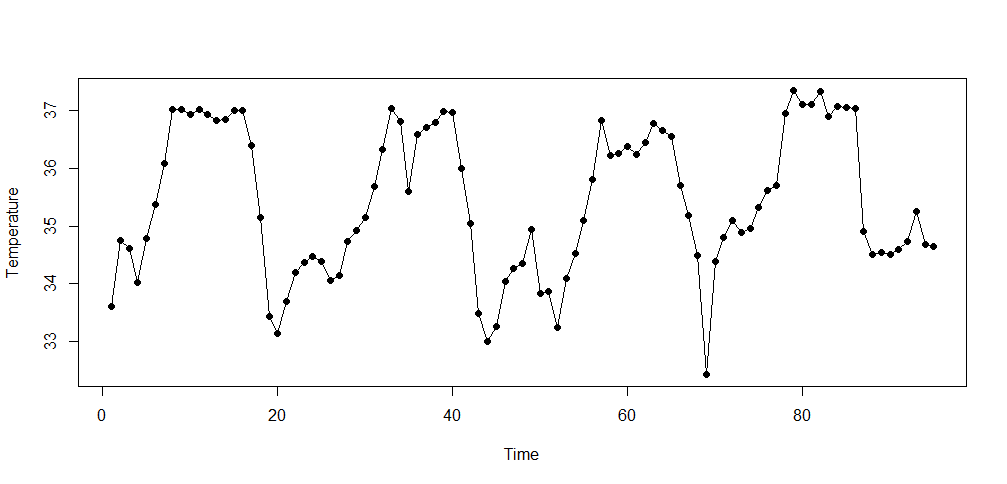
\includegraphics[scale = 0.3]{Temp8.png}
	\caption{Time series of the temperature of patient 8.}
	\label{fig:Temp8}
\end{figure}

The periodicity of this time series suggests applying an harmonic regression to fit the data. The first step for working on spectral analysis is considering a zero mean process. Therefore, we performed our analysis on the residuals, by subtracting the trend. 

In order to find the frequencies that drive the data, we explored the periodogram; notice that it is recommended to investigate behaviours of the \text{smoothed} periodogram, which is a \textit{consistent} estimator of the spectral density function. 

In Figure \ref{fig:period_Temp8}, we show the periodogram for this time series, and two different smoothing version of it, using uniform weights and \textit{Daniell} weights. We can notice how the main frequency which drives the data is around 0.04, i.e 1/24 hours.

\begin{figure}[htbp]\centering
	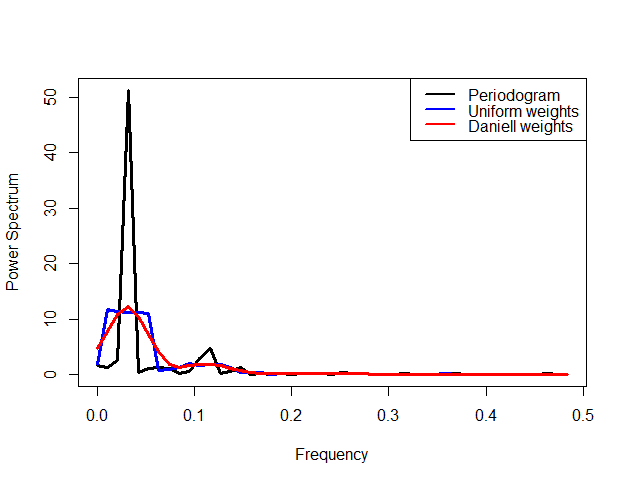
\includegraphics[scale = 0.4]{Temp8_Periodograms.png}
	\caption{Periodogram and smoothed periodograms (uniform and Daniell weights) for temperature of patient 8. This figure is best viewed in colours.}
	\label{fig:period_Temp8}
\end{figure}

\vspace{0.1cm}
Furthermore, it can be shown that the spectrum of any (weakly) stationary time series can be approximated through the spectrum of an AR($p$) model, whose explicit form is known. In order to find the \textit{best} lag parameter $p$ we fit several AR($p$) to the data, for increasing values of $p$. We then calculated two measures of quality of the model, BIC and AIC; the smallest value for BIC or AIC is a good suggestion for choosing the value of $p$. We give in Figure \ref{fig:spectrums_Temp8} an idea of this procedure to find the value of $p$; hence, we show the spectrum of an AR(2) and AR(9). 

\begin{figure}[htbp]
	\centering
	\subfigure[AIC and BIC]{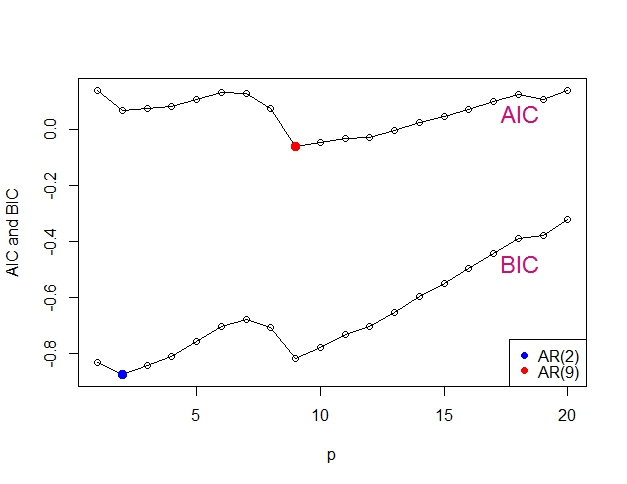
\includegraphics[scale = 0.32]{Temp8_AIC_BIC.png}}
	\subfigure[Spectrum AR(2), AR(9)]{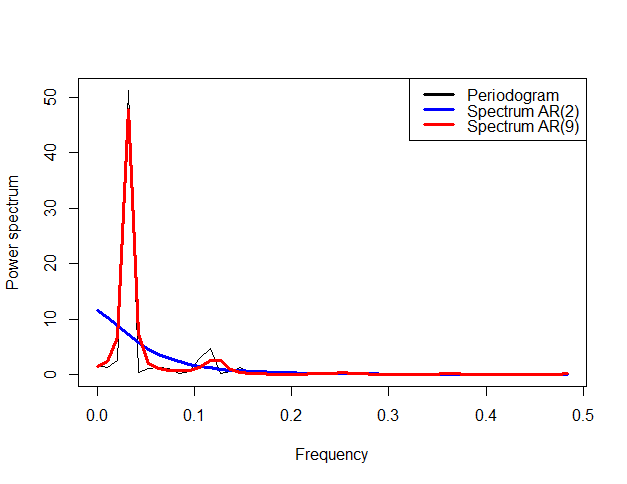
\includegraphics[scale = 0.32]{Temp8_AR_spectrums.png}}
	\hfill
	\caption{AR($p$) approach to obtain the correct frequency representation. Main frequencies that drive the data are around 1/24, and 1/8}
	\label{fig:spectrums_Temp8}
\end{figure}

Once the correct frequencies are selected, we can apply the harmonics regression explained in Section 1.1. The resulting model is given in Figure \ref{fig:fitted.Temp8}, where we used a total of 5 harmonics. As we stated before, the main frequency that drives the data results in a period of 24 hours

\begin{figure}[htbp]\centering
	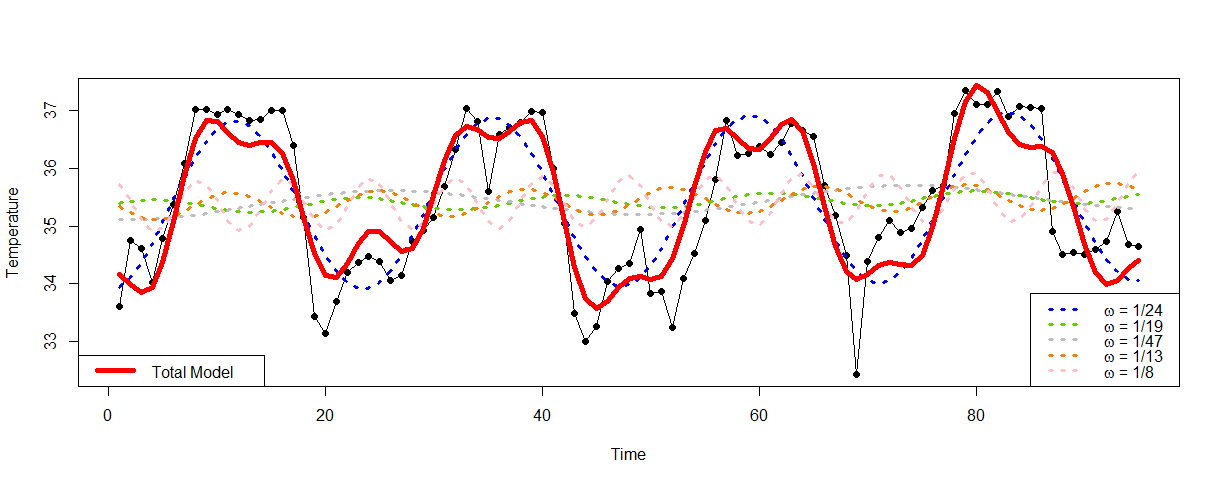
\includegraphics[scale = 0.37]{fitted_temp8.png}
	\caption{Harmonic regression for temperature of patient 8, using 5 different harmonics. Dotted lines represent the fitting for single harmonics; thick red line is the superposition of the dotted harmonics, which is the final fit.}
	\label{fig:fitted.Temp8}
\end{figure}

\vspace{1cm}
Finally, we give a 24 hour forecast in Figure \ref{fig:forecast.Temp8}

\begin{figure}[htbp]\centering
	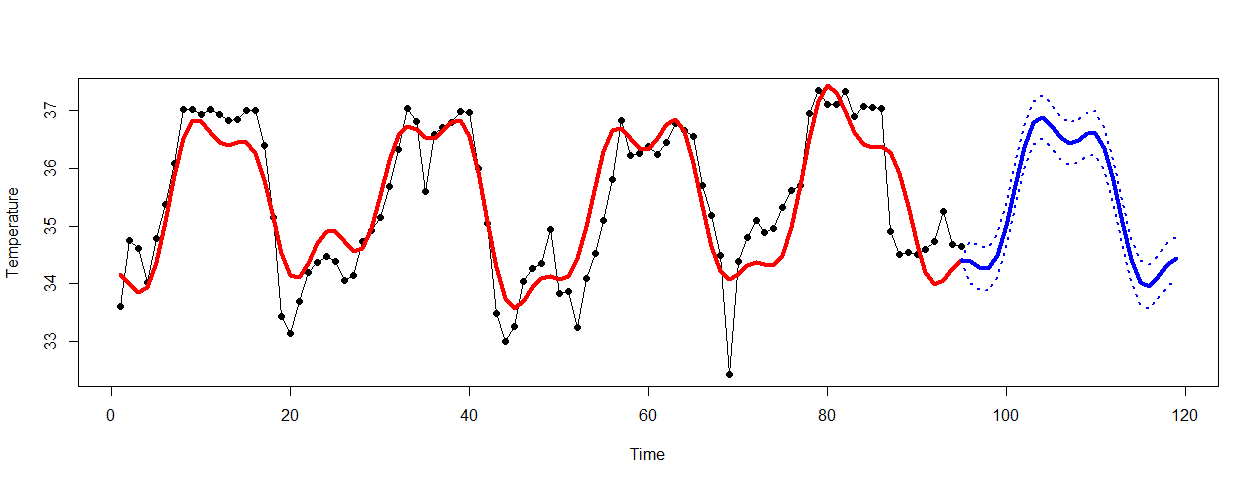
\includegraphics[scale = 0.37]{forecasting_Temp8.png}
	\caption{24 hour forecast for temperature of patient 8.}
	\label{fig:forecast.Temp8}
\end{figure}



\subsubsection*{Rest Activity}
The second time series we analyse is the rest activity, which is measured through an accelerometer placed on the chest of the patient. This data takes a particular shape as it take value zero when the patient is resting, and a continuous range of positive values when he is not resting. Therefore, fitting an harmonic regression appears to be difficult and probably not the best choice. However, we give in  Figure \ref{fig:fit_restactivity.temp8} the harmonic fitting using 5 harmonics; in the same figure we show an alternative model where we put an indicator function to the fitted values: negative values are taken to be zero. 

\begin{figure}[htbp]\centering
	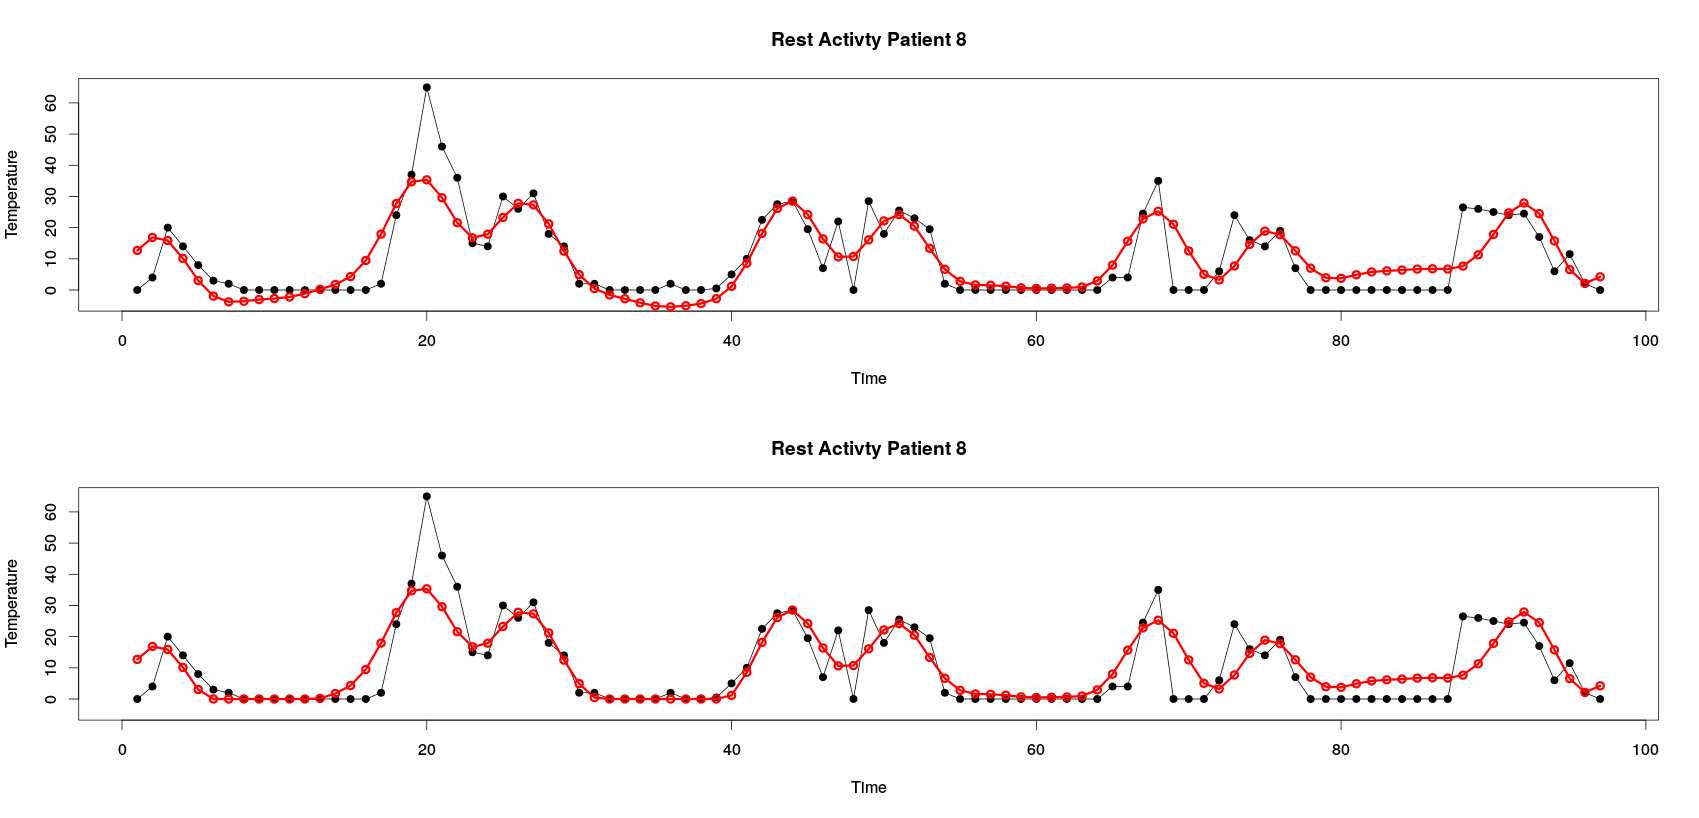
\includegraphics[scale = 0.22]{fit_rest_activty_Patient_8.png}
	\caption{Harmonic regression for rest activity of patient 8, using 5 harmonics. On top it is shown the classic harmonic fitting, whereas on the bottom the alternative model. }
	\label{fig:fit_restactivity.temp8}
\end{figure}


\subsubsection*{Testing models}
We now turn on testing the models we fit for both temperature and rest activity. In order to do so, we split our data in 3 days of training, and 1 day of testing; to measure the accuracy of our prediction we use standard mean square error (MSE). We summarise this in Table \ref{table:test.Temp} and Table \ref{table:test.Temp}

\begin{table}[htbp]
\begin{center}
\begin{tabular}{ ccc } 
 Data & MSE & N. Harmonics \\
  \hline
 Temp2 & 1.92 & 5 \\
 Temp8 & 0.58 & 5\\
 Temp24& 0.27 & 7\\
 Temp26& 0.43 & 3\\
\end{tabular}
\end{center}
\caption{MSE for temperature. 3 days training, 1 day testing.}
\label{table:test.Temp}
\end{table}


\begin{table}[htbp]
\begin{center}
\begin{tabular}{ ccc } 
 Data & MSE & N.Harmonics \\
  \hline
 RA2 & 430.64 & 5 \\
 RA8 & 308.60 & 5\\
 RA24& 398.23 & 6\\
 RA26& 577.91 & 5\\
\end{tabular}
\end{center}
\caption{MSE for rest activity. 3 days training, 1 day testing.}
\label{table:test.RA}
\end{table}


\end{document}


